\let\negmedspace\undefined
\let\negthickspace\undefined
\documentclass[journal]{IEEEtran}
\usepackage[a5paper, margin=10mm, onecolumn]{geometry}
\usepackage{lmodern} % Ensure lmodern is loaded for pdflatex
\usepackage{tfrupee} % Include tfrupee package

\setlength{\headheight}{1cm} % Set the height of the header box
\setlength{\headsep}{0mm}     % Set the distance between the header box and the top of the text

\usepackage{gvv-book}
\usepackage{gvv}
\usepackage{cite}
\usepackage{amsmath,amssymb,amsfonts,amsthm}
\usepackage{algorithmic}
\usepackage{graphicx}
\usepackage{textcomp}
\usepackage{xcolor}
\usepackage{txfonts}
\usepackage{listings}
\usepackage{enumitem}
\usepackage{mathtools}
\usepackage{gensymb}
\usepackage{comment}
\usepackage[breaklinks=true]{hyperref}
\usepackage{tkz-euclide} 
\usepackage{listings}                                      
\def\inputGnumericTable{}                                 
\usepackage[latin1]{inputenc}                                
\usepackage{color}                                            
\usepackage{array}                                            
\usepackage{longtable}
\usepackage{multicol}
\usepackage{calc}                                             
\usepackage{multirow}                                         
\usepackage{hhline}                                           
\usepackage{ifthen}                                           
\usepackage{lscape}
\begin{document}
	
	\bibliographystyle{IEEEtran}
	\vspace{3cm}
	
	\title{11.16.3.3.3}
	\author{EE24BTECH11030 - KEDARANANDA }
	% \maketitle
	% \newpage
	% \bigskip
	{\let\newpage\relax\maketitle}
	
	\renewcommand{\thefigure}{\theenumi}
	\renewcommand{\thetable}{\theenumi}
	\setlength{\intextsep}{10pt} % Space between text and floats
	
	
	\numberwithin{equation}{enumi}
	\numberwithin{figure}{enumi}
	\renewcommand{\thetable}{\theenumi}
	
	
	\textbf{Question}:\\
	A die is rolled. Find the probability that a number greater than or equal to one will appear.\\
	\textbf{Solution: }\\
	\textbf{Theoretical solution: }\\
	\[
	\text{Total outcomes} = 6.
	\]
	\[
	\text{Favorable outcomes} = 6.
	\]
	\[
	P(\text{Number} \geq 1) = \frac{\text{Favorable outcomes}}{\text{Total outcomes}} = \frac{6}{6} = 1.
	\]
	
	\textbf{Computational solution: }\\
	The PMF for a fair die is:
	\begin{align}
		P(X = x) =
		\begin{cases}
			\frac{1}{n}, & k \in \{1, 2,\dots ,n\} \\
			0, & \text{otherwise}
		\end{cases}
	\end{align}	
	\subsection*{Conclusion}
	The probability of rolling a number greater than or equal to one is the sum of all PMF values:
	\begin{align}
		P(X \geq 1) = \sum_{k=1}^{6} P_X(k) = \frac{6}{6} = 1.
	\end{align}
	\subsection*{Cumulative Distribution Function (CDF)}
	
	The cumulative distribution function (CDF) \(F(x)\) of a discrete random variable \(X\), representing the outcome of a die roll, is defined as:\\
	The CDF for the die roll is:
	\begin{align}
		F_X(k) = P(X \leq k) =
		\begin{cases}
			0, & k < 1 \\
			\frac{k}{n}, & 1 \leq k < n\\
			1, & k \geq n
		\end{cases} \label{cdf}
	\end{align}
	Where n is 6. \\ 
	$\therefore$ probability that a number greater than or equal to one will
	appear is ; from \eqref{cdf}
	\begin{align}
		P(X \geq 1) = 1 - F(X < 1) = 1
	\end{align} 
	
	\begin{figure}[h!]
		\centering
		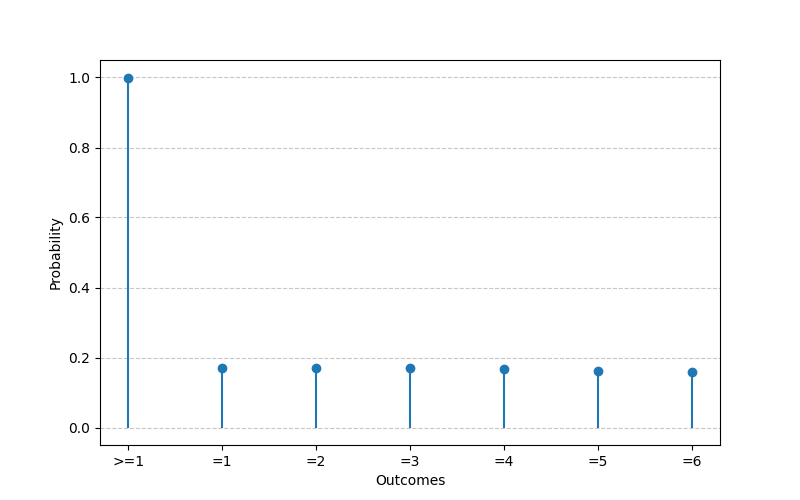
\includegraphics[width=\columnwidth]{figs/Fig.png}
		\label{stemplot}
	\end{figure}
	
\end{document}
